\subsection{Problembeschreibung}

Das Projekt beschäftigt sich mit den Eigenschwingeungen einer fest eingespannten Saite. Sei dazu $u(t, x)$ die vertikale Auslenkung der Saite an der Position $x \in [0, 1]$ zur Zeit $t$. $u$ wird näherungsweise durch die sogenannte Wellengleichung

\begin{align} \label{Wellengleichung}
  \frac{\partial^2 u}{\partial x^2} (t, x) =
  \frac{1}{c^2}
  \frac{\partial^2 u}{\partial t^2} (t, x)
\end{align}

für alle $x \in (0, 1)$ und $t \in \R$ beschrieben, wobei $c$ die Ausbreitungsgeschwindigkeit der Welle ist. Wenn die Saite an beiden Enden fest eingespannt ist, so gelten die Randbedingungen

\begin{align*}
  u(t, 0) = u(t, 1) = 0
\end{align*}

für alle $t \in \R$. \\

Zur Berechnung der Eigenschwingungen suchen wir nach Lösungen $u$, die in der Zeit harmonisch schwingen. Solche erfüllen folgenden Ansatz

\begin{align*}
  u(x, t) = \Re (v(x) e^{-i \omega t})
\end{align*}

mit einer festen, aber unbekannten Kreisfrequenz $\omega > 0$ und einer Funktion $v$, welche nur noch vom Ort $x$ abhängt. Durch Einsetzen erhalten wir für $v$ die sogenannte Helmholz-Gleichung

\begin{align} \label{Helmholz-Gleichung}
  -v^\primeprime(x) = \kappa^2 v(x), \qquad
  x \in (0, 1),
\end{align}

mit der unbekannten Wellenzahl $\kappa := \frac{\omega}{c}$ und den Randbedingungen

\begin{align} \label{Randbedingungen}
  v(0) = v(1) = 0.
\end{align}

\subsection{Analytische Lösung}

\begin{align}
  v_\kappa(x) = C_1 \cos{(\kappa x)} + C_2 \sin{(\kappa x)}, \qquad
  x \in [0, 1],
  \label{Analytische_Lösung}
\end{align}

mit beliebigen Konstanten $C_1, C_2$, löst die Helmholz-Gleichung \eqref{Helmholz-Gleichung}. Das erkennt man durch stumpfes Einsetzen.

\begin{multline*}
  - v_\kappa^\primeprime(x)
  = - \frac{\partial^2}{\partial x^2}
    (C_1 \cos{(\kappa x)} + C_2 \sin{(\kappa x)})
  = - \frac{\partial}{\partial x}
    (- C_1 \kappa \sin{(\kappa x)} + C_2 \kappa \cos{(\kappa x)}) \\
  = - (- C_1 \kappa^2 \cos{(\kappa x)} - C_2 \kappa^2 \sin{(\kappa x)})
  = \kappa (C_1 \cos{(\kappa x)} + C_2 \sin{(\kappa x)})
  = \kappa^2 v_\kappa(x)
\end{multline*}

Wir fragen uns, für welche $\kappa > 0$, Konstanten $C_1$ und $C_2$ existieren, sodass $v_\kappa$ auch die Randbedingungen \eqref{Randbedingungen} erfüllt.

\begin{align*}
  0 \stackrel{!}{=}
  \begin{cases}
    v_\kappa(0)
    = C_1 \cos{(0)} + C_2 \sin{(0)}
    = C_1 \\
    v_\kappa(1)
    = C_1 \cos{(\kappa)} + C_2 \sin{(\kappa)}
    = C_2 \sin{(\kappa)}
  \end{cases}
\end{align*}

Nachdem $\cos{(0)} = 1$ und $\sin{(0)} = 0$ erhält man aus der oberen Gleichung $C_1 = 0$. Mit der unteren Gleichung folgt aber auch $C_2 \sin{(\kappa)} = 0$. Wenn nun auch $C_2 = 0$, dann erhielte man die triviale Lösung $v_\kappa = 0$. Für eine realistischere Modellierung, d.h. $v_\kappa \neq 0$, müsste $\sin{(\kappa)} = 0$, also $\kappa \in \pi \Z$. \\

Das sind die gesuchten $\kappa > 0$. Sei nun eines dieser $\kappa$ fest. Offensichtlich ist $C_1 = 0$ eindeutig, $C_2 \in \R$ jedoch beliebig.

\subsection{Numerische Approximation}

Häufig lassen sich solche Probleme nicht analytisch lösen, sodass auf numerische Verfahren zurückgegriffen wird, welche möglichst gute Näherungen an die exakten Lösungen berechnen sollen. Als einfachstes Mittel dienen sogenannte Differenzenverfahren. Sei dazu $x_j := jh$, $j = 0, \ldots, n$ eine Zerlegung des Intervalls $[0, 1]$ mit äquidistanter Schrittweite $h = 1/n$. Die zweite Ableitung in \eqref{Helmholz-Gleichung} wird approximiert durch den Differenzenquotienten

\begin{align} \label{Differenzenquotient}
  v^\primeprime(x_j) \approx
  D_h v(x_j) :=
  \frac{1}{h^2} (v(x_{j-1}) - 2 v(x_j) + v(x_{j+1})), \qquad
  j = 1, \ldots, n-1.
\end{align}

Es sei angemerkt, dass \eqref{Differenzenquotient} tatsächlich einen Differenzenquotienten beschreibt. Um das einzusehen, verwenden wir den links- und rechts-seitigen Differenzenquotient erster Ordnung, sowie $x_{j-1} = x_j - h$, $x_{j+1} = x_j + h$. Wir erhalten $\Forall j = 1, \ldots, n-1:$

\begin{align*}
  v^\primeprime(x_j)
  & = \lim_{h \to 0}
      \Frac{h}
      {
        v^\prime(x_j + h) - v^\prime(x_j)
      } \\
  & = \lim_{h \to 0}
      \Frac{h}
      {
        \Frac{h}
        {
          v(x_j + h) - v(x_j)
        } -
        \Frac{h}
        {
          v(x_j) - v(x_j - h)
        }
      } \\
  & = \lim_{h \to 0}
      \Frac{h^2}
      {
        v(x_j + h) - 2 v(x_j) + v(x_j - h)
      } \\
  & = \lim_{h \to 0}
      D_h v(x_j)
\end{align*}

\subsubsection{Approximationsfehler}

Für hinreichend glatte Funktionen $v$ mit einer geeigneten Konstanten $C > 0$ wird der Approximationsfehler quadratisch in $h$ klein, d.h. dass

\begin{align} \label{quadratische_Konvergenz}
  \vbraces{v^\primeprime(x_j) - D_h v(x_j)} \leq C h^2.
\end{align}

Nachdem $v$ hinreichend glatt ist, gilt nach dem Satz von Taylor, dass $\Forall j = 1, \ldots, n-1:$

\begin{align*}
  v(x_j + h) & =
  \sum_{\ell = 0}^{n+2}
  \frac{h^\ell}{\ell !}
  v^{(\ell)}(x_j) +
  \Landau{h^{n+3}}, \\
  v(x_j - h) & =
  \sum_{\ell = 0}^{n+2}
  \frac{(-h)^\ell}{\ell !}
  v^{(\ell)}(x_j) +
  \Landau{h^{n+3}}.
\end{align*}

Man beachte, dass sich die ungeraden Summanden, der oberen Taylor-Polynome, gegenseitig aufheben. Damit erhalten wir für den Differenzenquotient $D_h v(x_j)$, $j = 1, \ldots, n-1$ eine asymptotische Entwicklung.

\begin{align*}
  D_h v(x_j)
  & = \Frac{h^2}
  {
    v(x_j - h) + v(x_j + h) - 2 v(x_j)
  } \\
  & = \Frac{h^2}
      {
        2 v(x_j) +
        h^2 v^\primeprime(x_j) +
        \sum_{\substack{\ell = 4 \\ \ell \in 2 \N}}^{n+2}
        \frac{h^\ell}{\ell !}
        v^{(\ell)}(x_j)
        (1 + (-1)^\ell) -
        2 v(x_j)
      } +
      \Landau{h^{n+3}} \\
  & = v^\primeprime(x_j) +
      2 \sum_{\ell = 1}^\floor{\frac{n}{2}}
      \frac{h^{2 \ell}}{(2 \ell + 2)!}
      v^{(2 \ell)}(x_j) +
      \Landau{h^{n+1}}
\end{align*}

Daraus folgt unmittelbar die quadratische Konvergenz \eqref{quadratische_Konvergenz}, d.h. $\Forall j = 1, \ldots, n-1:$

\begin{align*}
  D_h v(x_j) - v^\primeprime(x_j) = \Landau{h^2}, \qquad
  h \to 0.
\end{align*}

\subsubsection{Eigenwertproblem}

Wir wollen nun den Differenzenquotienten $D_h v(x_j)$ verwenden, um ein Eigenwertproblem der Form $A \mathbf{v} = \lambda \mathbf{v}$ mit einer Matrix $A \in \R^{(n-1) \times (n-1)}$ zu dem Eigenvektor $\mathbf{v} := (v(x_1), \ldots, v(x_{n-1}))^T$ und dem Eigenwert $\lambda := \kappa^2$ herzuleiten. Das soll die Helmholz-Gleichung \eqref{Helmholz-Gleichung}, mit Tupeln und Eigenwerten für die Funktionen $v_\kappa$ bzw. Vorfaktoren $\kappa$, approximieren. \\

Es wird eine Matrix $-A_n$, $n \geq 2$ gesucht, die den Differenzenquotienten $D_h v(x_j)$ auf den oberen Vektor $\mathbf{v}^{(n)}$ komponentenweise anwendet. Wir rufen in Erinnerung, dass $h = 1/n$ und definieren die naheliegende Matrix

\begin{align*}
  -A_n :=
  \frac{1}{h^2}
  \begin{pmatrix}
    -2 &  1      &        &    \\
     1 &  \ddots & \ddots &    \\
       &  \ddots & \ddots &  1 \\
       &         & 1      & -2
  \end{pmatrix}
  \in \R^{(n-1) \times (n-1)}.
\end{align*}

Wenn nun die Randbedingungen \eqref{Randbedingungen} gelten sollen, d.h. $v(x_0), v(x_n) = 0$, leistet diese Matrix $A_n$ tatsächlich das Gewünschte. Sie approximiert die linke Seite der Helmholz-Gleichung \eqref{Helmholz-Gleichung}.

\begin{align*}
  A_n \mathbf{v}^{(n)} =
  -\frac{1}{h^2}
  \begin{pmatrix}
    v(x_0) - 2 v(x_1) + v(x_2)             \\
    v(x_1) - 2 v(x_2) + v(x_3)             \\
    \vdots                                 \\
    v(x_{n-3}) - 2 v(x_{n-2}) + v(x_{n-1}) \\
    v(x_{n-2}) - 2 v(x_{n-1}) + v(x_{n-0})
  \end{pmatrix} =
  -\begin{pmatrix}
    D_h v(x_1) \\
    \vdots     \\
    D_h v(x_{n-1})
  \end{pmatrix}
  \xrightarrow{n \to \infty}
  -v^\primeprime
\end{align*}

Die Matrix $A_n$ wurde in der Funktion \verb|my_numpy_matrix| implementiert. \\

\newpage

\lstinputlisting
[language = Python]
{Aufgabe_2/python_code/my_numpy_matrix.py}
\vspace{10pt}

Das Eigenwertproblem wurde mit \verb|np.linalg.eig|, für beliebige $n \geq 2$, gelöst. \verb|np.linalg.eig| retourniert die Eigenwerte und Eigenvektoren nicht zwangsläufig, der größe der Eigenwerte nach, sortiert. Nachdem der Zusammenhang zwischen Eigenwert und Eigenvektor nicht verloren gehen soll, erfordert dies einigen logistischen Aufwand. Das ist aber nicht wesentlich und wird daher nicht weiter erklärt. Wir vergleichen lieber die Eigenwerte und Eigenvektoren mit den analytischen Ergebnissen. \\

In der folgenden Tabelle, sind die $3$ Eigenwerte (sollten diese bereits existieren), der Matrizen $A_2, \ldots, A_{10}$, aufgelistet. Diese Tabelle ist analog zu \eqref{Konvergenz_EW} zu verstehen. \\

\begin{tabular}{lrrrrrrrrr}
\toprule
{} &   2  &    3  &         4  &        5  &         6  &         7  &         8  &         9  &         10 \\
\midrule
1 &  8.0 &   9.0 &   9.372583 &   9.54915 &   9.646171 &   9.705051 &   9.743420 &   9.769795 &   9.788697 \\
2 &  NaN &  27.0 &  32.000000 &  34.54915 &  36.000000 &  36.897999 &  37.490332 &  37.900800 &  38.196601 \\
3 &  NaN &   NaN &  54.627417 &  65.45085 &  72.000000 &  76.192948 &  79.016521 &  81.000000 &  82.442950 \\
\bottomrule
\end{tabular}

\vspace{10pt}

Die Matrix $A_n$ besitzt also scheinbar $n-1$ paarweise verschiedene Eigenwerte $\lambda_{1, n} < \cdots < \lambda_{n-1, n}$, welche jeweils gegen $\lambda_i := (i \pi)^2$, $i \in \N$ konvergieren.

\begin{align} \label{Konvergenz_EW}
\begin{array}{ccccccccc}
\lambda_{1, 2} & \rightarrow & \lambda_{1, 3} & \rightarrow & \cdots & \rightarrow & \lambda_{1, n} & \xrightarrow{n \to \infty}   & \lambda_1 = (1 \pi)^2 \\
               &             & \lambda_{2, 3} & \rightarrow & \cdots & \rightarrow & \lambda_{2, n} & \xrightarrow{n \to \infty}   & \lambda_2 = (2 \pi)^2 \\
               &             &                &             & \ddots & \ddots      & \vdots         & \vdots                       & \vdots                \\
               &             &                &             &        &             & \lambda_{i, n} & \xrightarrow[n \to \infty]{} & \lambda_i = (i \pi)^2
\end{array}
\end{align}

Nachdem $\Bbraces{\sqrt{\lambda_i}: i \in \N_0} = \pi \N_0 \subsetneq \pi \Z$, könnte man sich nun fragen, wo die andere Hälfte der analytischen Ergebnisse steckt. Die Erklärung ist ganz unspektakulär $\lambda := (\pm \kappa)^2$. \\

Wir bezeichnen mit $\epsilon_i(n) := |\lambda_i - \lambda_{i, n}|$, $i = 1, \ldots, n-1$ den absoluten Konvergenz-Fehler des $i$-ten Eigenwertes. In der folgenden Abbildung \ref{fig:Konvergenz-Fehler_EW} wurde $\epsilon_i$ mit der Vergleich-Geraden $\id^2$, doppelt logarithmisch, geplottet. \\

\begin{figure}[H]
  \centering
  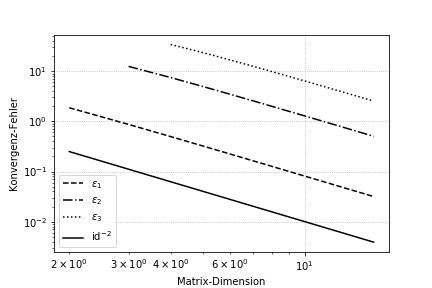
\includegraphics[width = 0.5 \textwidth]{Aufgabe_2/images/plot_eigen_value_errors(n_max = 16, i_max = 3)}
  \caption{Konvergenz-Fehler der Eigenwerte von $A_n$}
  \label{fig:Konvergenz-Fehler_EW}
\end{figure}

Allem Anschein nach, verschwindet $\epsilon_i$ quadratisch. Das korreliert mit dem Ergebnis \eqref{quadratische_Konvergenz}. Man beachte, dass der $i$-te Eigenwert erst ab einer Matrix $A_n$, $n > i$ existiert. Daher fangen die Plots von $\epsilon_i$ desto später an, je größer $i$ ist. Für größeres $i$ ist auch der intitiale Fehler größer. Obwohl dieser ebenfalls quadratisch konvergiert, werden mehr Rechenoperationen für ein genaues Ergebnis benötigt. \\

Seien $\mathbf{v}^{(1, n)}, \ldots, \mathbf{v}^{(n-1, n)}$ die Eigenvektoren (modulo Konstante), zu den Eigenwerten $\lambda_{1, n} < \cdots < \lambda_{n-1, n}$, der Matrix $A_n$. Diese sollten nun gegen die Funktionen $v_{\kappa_i}$, $\kappa_i = \sqrt{\lambda_i}$, vielleicht sogar quadratisch, konvergieren. Die folgende Abbildung \ref{fig:Eigenvektoren} soll dies veranschaulichen.

\begin{figure}[H]
  \centering
  \subfloat[Eigenvektoren $\mathbf{v}^{(1, n)}$, $n = 2, 4, 8, 32$]{
    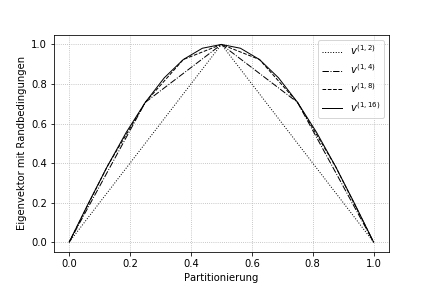
\includegraphics[width=65mm]{Aufgabe_2/images/plot_eigen_vectors/plot_eigen_vectors(n_array = [2, 4, 8, 16], i = 1).png}
  }
  \subfloat[Eigenvektoren $\mathbf{v}^{(2, n)}$, $n = 4, 8, 16, 64$]{
    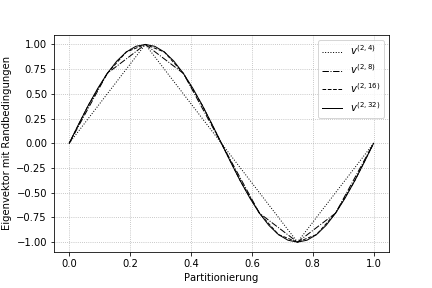
\includegraphics[width=65mm]{Aufgabe_2/images/plot_eigen_vectors/plot_eigen_vectors(n_array = [4, 8, 16, 32], i = 2).png}
  }
  \hspace{0mm}
  \subfloat[Eigenvektoren $\mathbf{v}^{(3, n)}$, $n = 8, 16, 32, 64$]{
    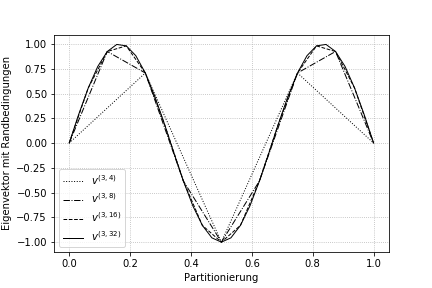
\includegraphics[width=65mm]{Aufgabe_2/images/plot_eigen_vectors/plot_eigen_vectors(n_array = [4, 8, 16, 32], i = 3).png}
  }
  \subfloat[Eigenvektoren $\mathbf{v}^{(4, n)}$, $n = 8, 16, 32, 64$]{
    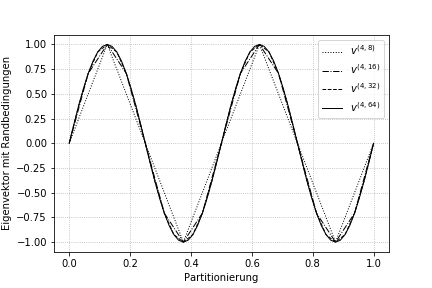
\includegraphics[width=65mm]{Aufgabe_2/images/plot_eigen_vectors/plot_eigen_vectors(n_array = [8, 16, 32, 64], i = 4).png}
  }
  \hspace{0mm}
  \caption{Eigenvektoren $\mathbf{v}^{(i, n)}$, $i = 1, \ldots, 4$ der Matrizen $A_n$}
  \label{fig:Eigenvektoren}
\end{figure}

Erstaunlicherweise, gibt es scheinbar keinen Konvergenz-Fehler, da die Eigenvektoren direkt an den Grenzfunktionen liegen. Mit anderen Worten, $\Forall n \in \N, \Forall i, j = 1, \ldots n-1:$

\begin{align*}
  \mathbf{v}^{(i, n)}_j = v_{\kappa_i}(x_j).
\end{align*}

Anschaulich, erhält man ein zu \eqref{Konvergenz_EW} analoges Schema \eqref{Konvergenz_EV}.

\begin{align} \label{Konvergenz_EV}
\begin{array}{ccccccccc}
\mathbf{v}^{(1, 2)} & \rightarrow & \mathbf{v}^{(1, 3)} & \rightarrow & \cdots & \rightarrow & \mathbf{v}^{(1, n)} & \xrightarrow{n \to \infty}   & v_{\kappa_1} \\
                &             & \mathbf{v}^{(2, 3)} & \rightarrow & \cdots & \rightarrow & \mathbf{v}^{(2, n)} & \xrightarrow{n \to \infty}   & v_{\kappa_2} \\
                &             &                 &             & \ddots & \ddots      & \vdots          & \vdots                       & \vdots       \\
                &             &                 &             &        &             & \mathbf{v}^{(i, n)} & \xrightarrow[n \to \infty]{} & v_{\kappa_i}
\end{array}
\end{align}

\subsection{Verallgemeinerte Problembeschreibung}

Die Ausbreitungsgeschwindigkeit $c$ in \eqref{Wellengleichung} hängt vom Material der Saite ab. Bisher haben wir sie als konstant angenommen, d.h. die Saite bestand aus einem Material. Sei nun für $c_0, c_1 \in \R$

\begin{align} \label{Material-Funktion}
  c(x) :=
  \begin{cases}
    c_0, x \in (0, 1/2) \\
    c_1, x \in (1/2, 1)
  \end{cases}.
\end{align}

\subsection{Verallgemeinerte Analytische Lösung}

Zuerst leiten wir eine zur Helmholz-Gleichung \eqref{Helmholz-Gleichung} ähnliche Gleichung her und geben einen \eqref{Analytische_Lösung} entsprechenden Lösungsansatz an, wenn die Lösung $v$ auf $(0, 1)$ stetig differenzierbar sein soll.
Dabei betrachten wir eine angepasste Version der Wellengleichung \eqref{Wellengleichung}.

\begin{align*}
  \frac{\partial^2 u}{\partial x^2} (t, x) =
  \frac{1}{c^2(x)}
  \frac{\partial^2 u}{\partial t^2} (t, x), \qquad
  x \in (0, 1), \qquad
  t \in \R
\end{align*}

Wir verwenden jedoch den selben Ansatz, wie Vorher. Das war $u(x, t) = \Re (v(x) e^{-i \omega t})$, mit einer festen, aber unbekannten Kreisfrequenz $\omega > 0$ und einer Funktion $v$, welche nur noch vom Ort $x$ abhängt. \\

Einsetzen und analoges Nachrechnen, gibt, mit der unbekannten Wellenzahl $\kappa(x) := \frac{\omega}{c(x)}$, die Randbedingungen \eqref{Randbedingungen} und

\begin{align*}
  -v^\primeprime(x) = \kappa^2(x) v(x), \qquad
  x \in (0, 1).
\end{align*}

Um Probleme mit der Differenzierbarkeit von $\kappa$ zu vermeiden, führen wir die Abkürzungen $\kappa_0 := \frac{\omega}{c_0}$, $\kappa_1 := \frac{\omega}{c_1}$ ein, und definieren den Lösungsansatz durch Fallunterscheidung und mit (vorerst) beliebigen Konstanten $C_{01}, C_{02}, C_{11}, C_{12}$.

\begin{align*}
  v(x) :=
  \begin{cases}
    C_{01} \cos{(\kappa_0 x)} + C_{02} \sin{(\kappa_0 x)},
    & x \in (0, 1/2) \\
    C_{11} \cos{(\kappa_1 x)} + C_{12} \sin{(\kappa_1 x)},
    & x \in (1/2, 1)
  \end{cases}
\end{align*}

Durch Berücksichtigung der Randbedingungen \eqref{Randbedingungen}, erhält man (fast analog zu Vorher)

\begin{align*}
  C_{01} = 0, \qquad
  C_{11} \cos{(\kappa_1)} + C_{12} \sin{(\kappa_1)} = 0.
\end{align*}

Soll $v$ auf $1/2$ stetig fortgesetzt werden, so müssen dessen links- und rechts-seitiger Grenzwert übereinstimmen.

\begin{align*}
  C_{02} \sin(\kappa_0/2)
  = \lim_{x \to 1/2-} v(x)
  = \lim_{x \to 1/2+} v(x)
  = C_{11} \cos(\kappa_1/2) + C_{12} \sin(\kappa_1/2)
\end{align*}

Um stetige Differenzierbarkeit zu erhalten, muss auch die Ableitung

\begin{align*}
  v^\prime(x) =
  \begin{cases}
    C_{02} \kappa_0 \cos(\kappa_0 x),
    & x \in (0, 1/2) \\
    - C_{11} \kappa_1 \sin(\kappa_1 x) + C_{12} \kappa_1 \cos(\kappa_1 x),
    & x \in (1/2, 1)
  \end{cases}
\end{align*}

auf $1/2$ stetig fortgesetzt werden.

\begin{align*}
  C_{02} \kappa_0 \cos(\kappa_0/2)
  = \lim_{x \to 1/2-} v^\prime(x)
  = \lim_{x \to 1/2+} v^\prime(x)
  = - C_{11} \kappa_1 \sin(\kappa_1/2) + C_{12} \kappa_1 \cos(\kappa_1/2)
\end{align*}

Aus den Randbedingungen und stetigen Fortsetzungen, ergibt sich also das homogene lineare Gleichungssystem $R \mathbf{C} = 0$, mit

\begin{align*}
  R :=
  \begin{pmatrix}
    \sin(\kappa_0/2)          & -\cos(\kappa_1/2)         & -\sin(\kappa_1/2) \\
    \kappa_0 \cos(\kappa_0/2) & \kappa_1 \sin(\kappa_1/2) & - \kappa_1 \cos(\kappa_1/2) \\
    0                         & \cos{\kappa_1}            & \sin{\kappa_1}
  \end{pmatrix}
  \in \R^{3 \times 3}, \qquad
  \mathbf{C} :=
  \begin{pmatrix}
    C_{02} \\
    C_{11} \\
    C_{12}
  \end{pmatrix}
  \in \R^{3 \times 1}.
\end{align*}

Sei $R \in \GL[3]{\R}$ regulär, so ist deren Kern trivial, d.h. $\ker{R} = \Bbraces{0}$, und somit auch die Lösung $\mathbf{C} = 0$. Dieser Trivialfall wurde jedoch vorhin bereits ausgeschlossen. Darum betrachten wir $\det{R} = 0$. Mit SymPy berechnet man

\begin{align} \label{Nullfunktion}
  \nonumber
  \det{R}
  & = \sin{\left(\frac{{\kappa}_{0}}{2} \right)} \cos{\left(\frac{{\kappa}_{1}}{2} \right)} {\kappa}_{1} + \sin{\left(\frac{{\kappa}_{1}}{2} \right)} \cos{\left(\frac{{\kappa}_{0}}{2} \right)} {\kappa}_{0} \\
  & = \sin{\pbraces{\frac{\omega}{2 c_0}}}
      \cos{\pbraces{\frac{\omega}{2 c_1}}}
      \frac{\omega}{c_1} +
      \sin{\pbraces{\frac{\omega}{2 c_1}}}
      \cos{\pbraces{\frac{\omega}{2 c_0}}}
      \frac{\omega}{c_0} =: f_c(\omega)
\end{align}

Für feste $c_0$, $c_1$, lässt sich das gewünschte $\omega$, als (nicht eindeutige) Nullstelle dieser Funktion $f_c$, charakterisieren.

\subsection{Verallgemeinerte Semi-Analytische Lösung}

Das Ergebnis aus \eqref{Nullfunktion} wurde, in Form von folgender Funktion, implementiert. \\

\lstinputlisting
[language = Python]
{Aufgabe_2/python_code/get_zero_function.py}
\vspace{10pt}

Nun können wir $f_c$ für fixe $c_0, c_1$ plotten lassen. Dann bekommen wir ein besseres Verständnis dafür, welchen Startwert wir wählen sollen, um die Gleichung $f_c(\omega) = 0$, mit \verb|scipy.optimize.fsolve| lösen zu lassen. \\

Für die folgenden Plots in Abbildung \ref{fig:zero_function}, wurden die arbiträren Werte $c_0 = 100$, $c_1 = 1$ gewählt. Die davon abhängige Funktion $f_c$ ist scheinbar gerade. Das liegt an \eqref{Nullfunktion}, sowie dass $\cos$ gerade und $\sin$ ungerade ist.


\begin{figure}[H]
  \centering
  \subfloat[auf dem Intervall $(-16, 16)$]{
    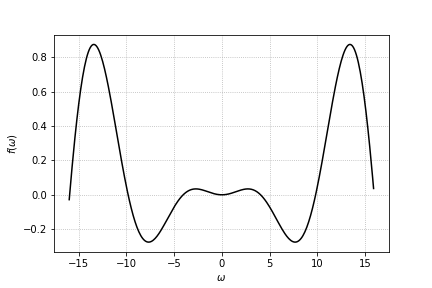
\includegraphics[width=65mm]{Aufgabe_2/images/plot_omegas/plot_omegas(c = (100, 1), interval = (-16, 16))}
  }
  \subfloat[auf dem Intervall $(0, 30)$ und herangezoomt]{
    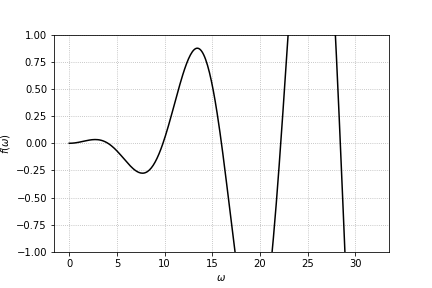
\includegraphics[width=65mm]{Aufgabe_2/images/plot_omegas/plot_omegas(c = (100, 1), interval = (0, 32), limits = (-1, 1))}
  }
  \hspace{0mm}
  \caption{Plots von $f_c$ für $c_0 = 100$, $c_1 = 1$}
  \label{fig:zero_function}
\end{figure}

Dementsprechend, können passende Startwerte $\tilde{\omega}$ für iterative Verfahren gewählt werden. Die jeweils ersten Ergebnisse $\omega$ vom, bereits erwähnten, \verb|scipy.optimize.fsolve| sind in der folgenden Tabelle zu sehen. Die Quadrate $\omega^2$ dieser Ergebnisse sind Approximationen der Grenzwerte der Eigenwerte, die wir im nächsten Unterkapitel betrachten. \\
\begin{center}

\begin{tabular}{lrrrrrr}
\toprule
{} &          1 &          2 &           3 &           4 &           5 &           6 \\
\midrule
$\tilde \omega$ &   5.000000 &  10.000000 &   15.000000 &   20.000000 &   25.000000 &   30.000000 \\
$\omega$        &   4.057425 &   9.826058 &   15.956815 &   22.170349 &   15.956815 &   28.413934 \\
$\omega^2$      &  16.462695 &  96.551423 &  254.619961 &  491.524375 &  254.619961 &  807.351663 \\
\bottomrule
\end{tabular}

\vspace{10pt}
\end{center}

\subsection{Verallgemeinertes Eigenwertproblem}

Wir wollen nun den Differenzenquotienten $D_h v(x_j)$ verwenden, um ein verallgemeintertes Eigenwertproblem der Form $A \mathbf{v} = \lambda B \mathbf{v}$ mit Matrizen $A, B \in \R^{(n-1) \times (n-1)}$ herzuleiten. \\

Sei abermals $x_j := jh$, $j = 0, \ldots, n$ unsere Zerlegung des Intervalls $[0, 1]$ mit äquidistanter Schrittweite $h = 1/n$. Die Matrix $-A_n$, für den Differenzenquotienten $D_h v(x_j)$, und der Vektor $\mathbf{v}^{(n)} := (v(x_1), \ldots, v(x_{n-1}))^T$, bleiben ebenfalls nach wie vor so, wie sie waren. \\

$B_n \lambda$ soll nun, analog zu Vorher, $\kappa^2$ repräsentieren. Diesmal, ist $\kappa$ jedoch als (stückweise konstante) Funktion zu verstehen. Also wird die Matrix $B_n$ deren Fallunterscheidungen übernehmen und $\lambda$ konstant bleiben. Es läuft darauf hinaus, dass \\

\begin{align*}
  B_n :=
  \begin{cases}
    \diag^{-2}
    (
      c_0, \ldots, c_0,
      c_1, \ldots, c_1,
    ), & n-1 \in 2 \N \\
    \diag^{-2}
    (
      c_0, \ldots, c_0,
      \frac{c_0 + c_1}{2},
      c_1, \ldots, c_1,
    ), & n-1 \in 2 \N + 1
  \end{cases},
  \qquad
  \lambda := \omega^2,
\end{align*}

wobei $c_0, c_1$ in $B_n \in \GL[n-1]{\R}$ jeweils $\floor{\frac{n-1}{2}}$-mal vorkommen. Dabei sei vorausgesetzt, dass $c_0, c_1 \neq 0$ und $c_0 + c_1 \neq 0$. Die Wahl von $B_n$ lässt sich wie folgt begründen. \\

Seien $\mathbf{a}, \mathbf{b}$ Vektoren mit gleich vielen Komponenten. Dann ist die Matrix-Vektor-Multiplikation $\cdot$, mit einer erzeugten Diagonalmatrix, äquivalent zur komponentenweisen Multiplikaiton $\odot$.

\begin{align} \label{Diagonalmatrizen}
  \diag(\mathbf{a}) \cdot \mathbf{b} =
  \mathbf{a} \odot \mathbf{b} =
  \mathbf{b} \odot \mathbf{a} =
  \diag(\mathbf{b}) \cdot \mathbf{a}
\end{align}

Bei dem vorherigen Eigenwertproblem wäre $B_n$ als Einheits-Matrix $I_n$ zu interpretieren. Der Eigenwert $\lambda$ konnte gleich ganz $\kappa^2$ approximieren, weil dieser Wert konstant war. Man hätte aber freilich auch mit der Skalarmatrix $(I_n c)^{-2}$ und $\omega^2$ anstelle von $\kappa^2$ arbeiten können. Da $\kappa^2$ nun aber, als Funktion, zwei unterschiedliche Werte

\begin{align*}
  \pbraces{\frac{\omega}{c_0}}^2,
  \pbraces{\frac{\omega}{c_1}}^2
\end{align*}

annehmen kann, müssen wir die obere Eigenschaft \eqref{Diagonalmatrizen} von Diagonalmatrizen ausnutzen. Damit realisieren wir die Fallunterscheidung zwischen $x_j < 1/2$ und $x_j > 1/2$. Für $x_j = 1/2$, was genau bei $n-1 \in 2 \N$ auftritt, wird gemittelt. \\

Nachdem die Inverse einer Diagonalmatrix genau die Matrix selbst mit komponentenweise Kehrwerten ist, lassen sich gleich $B_n$ und $B_n^{-1}$ leicht implementieren. Die zuständigen Funktionen besitzen die kreativen Namen \verb|my_other_numpy_matrix| bzw. \verb|my_other_numpy_matrix_inverse|. \\

\lstinputlisting
[language = Python]
{Aufgabe_2/python_code/my_other_numpy_matrices.py}
\vspace{10pt}

Das verallgemeinerte Eigenwertproblem $A_n \mathbf{v} = \lambda B_n \mathbf{v}$ werden wir zunächst auf $B_n^{-1} A_n \mathbf{v} = \lambda \mathbf{v}$ umformulieren. Dieses kann nun ebenfalls mit \verb|np.linalg.eig|, für beliebige $n \geq 2$, gelöst werden. \\

Die Matrix $B_n^{-1} A_n$ besitzt hoffentilch wieder $n-1$ paarweise verschiedene Eigenwerte $\lambda^c_{1, n} < \cdots < \lambda^c_{n-1, n}$, die jeweils konvergieren. \\

Um einen ersten Eindruck des möglichen Konvergenz-Verhaltens zu bekommen, vergleichen wir die Eigenwerte mit den oberen semi-analytischen Ergebnissen mit $c_0 = 100$, $c_1 = 1$. Es folgt eine zur oberen analoge Tabelle mit Eigenwerten. Die Ergebnisse lassen zwar zu wünschen übrig, aber immerhin pendelt sich die Größenordnung rasch ein. \\

\begin{center}

\begin{tabular}{lrrrrr}
\toprule
{} &        2 &              3 &              4 &              5 &              6 \\
\midrule
1 &  20402.0 &      13.499662 &      21.329378 &      15.313793 &      20.048572 \\
2 &      NaN &  180004.500338 &   56813.374144 &      68.017688 &      96.940091 \\
3 &      NaN &            NaN &  344805.296478 &  250012.501563 &  102552.962302 \\
4 &      NaN &            NaN &            NaN &  750004.166956 &  422576.319931 \\
\bottomrule
\end{tabular}

\vspace{10pt}
\end{center}

Wir bezeichnen (optimistischerweise) mit $\epsilon_i^c(n) := |\lambda_i^c - \lambda_{i, n}^c|$, $i = 1, \ldots, n-1$ den absoluten Konvergenz-Fehler des $i$-ten Eigenwertes. $\lambda_i^c$ erhalten wir durch $\omega^2$ von \verb|scipy.optimize.fsolve|, wobei $\tilde{\omega} := \sqrt{\lambda_{i, n}^c}$ als Startwert für das iterative Verfahren gewählt wird. Theoretisch hängt $\lambda_i^c$ also noch von $n$ ab. In der folgenden Abbildung \ref{fig:Konvergenz-Fehler_EW_allgemein} wurde $\epsilon^c_i$ mit der Vergleich-Geraden $\id^2$, doppelt logarithmisch, geplottet. \\

\begin{figure}[H]
\centering
\subfloat[$c = (1, 1)$]{
  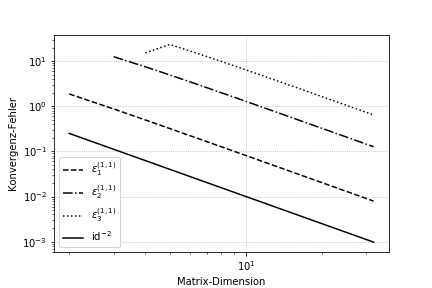
\includegraphics[width=65mm]{Aufgabe_2/images/plot_eigen_value_errors_general/plot_eigen_value_errors_general(n_max = 32, i_max = 3, c = (1, 1)).png}
  \label{subfig:Konvergenz-Fehler_EW}
}
\subfloat[$c = (1.1, 1)$]{
  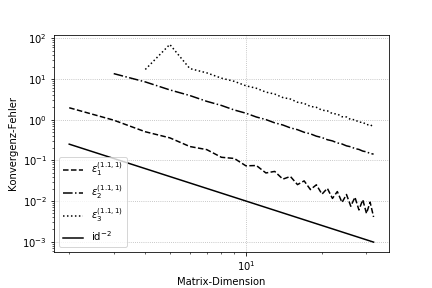
\includegraphics[width=65mm]{Aufgabe_2/images/plot_eigen_value_errors_general/plot_eigen_value_errors_general(n_max = 32, i_max = 3, c = (1.1, 1)).png}
}
\hspace{0mm}
\subfloat[$c = (2, 1)$]{
  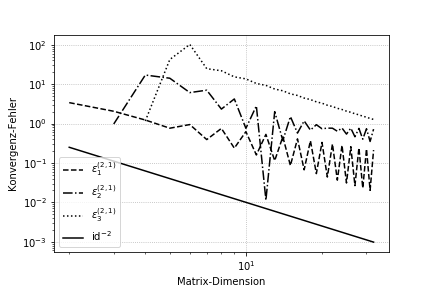
\includegraphics[width=65mm]{Aufgabe_2/images/plot_eigen_value_errors_general/plot_eigen_value_errors_general(n_max = 32, i_max = 3, c = (2, 1)).png}
  \label{Bergsteiger_a}
}
\subfloat[$c = (100, 1)$]{
  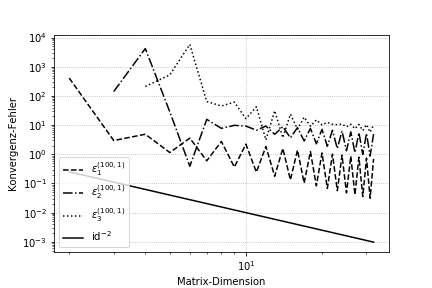
\includegraphics[width=65mm]{Aufgabe_2/images/plot_eigen_value_errors_general/plot_eigen_value_errors_general(n_max = 32, i_max = 3, c = (100, 1)).png}
  \label{Bergsteiger_b}
}
\hspace{0mm}
\caption{Konvergenz-Fehler der Eigenwerte von $B_n^{-1} A_n$, für $n = 2, \ldots, 32$ und}
\label{fig:Konvergenz-Fehler_EW_allgemein}
\end{figure}

Es macht Sinn, dass Abbildung \ref{subfig:Konvergenz-Fehler_EW} mit Abbildung \ref{fig:Konvergenz-Fehler_EW} korreliert. Diese \enquote{Bergsteiger-Konvergenz} steigt anscheinend mit dem Verhältnis $c_0/c_1$ (no pun intended). Etwas Aufschlussreicher werden \ref{Bergsteiger_a} und \ref{Bergsteiger_b}, wenn man gerade und ungerade $n$ unterscheidet. Diese Abbildung \ref{fig:Konvergenz-Fehler_EW_allgemein} bleibt übrigens unverändert, wenn man die Komponenten von $c$ vertauscht.


\begin{figure}[H]
\centering
\hspace{0mm}
\subfloat[$c = (2, 1)$, $n \in 2 \N$]{
  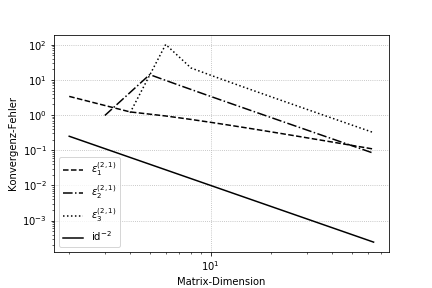
\includegraphics[width=65mm]{Aufgabe_2/images/plot_eigen_value_errors_general/plot_eigen_value_errors_general(n_max = 64, i_max = 3, c = (2, 1), parity = even).png}
}
\subfloat[$c = (100, 1)$, $n \in 2 \N$]{
  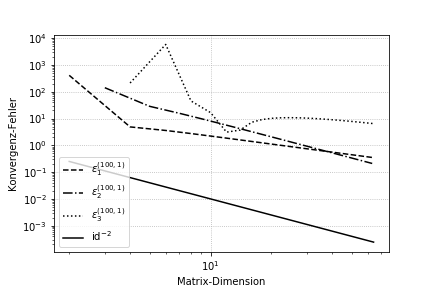
\includegraphics[width=65mm]{Aufgabe_2/images/plot_eigen_value_errors_general/plot_eigen_value_errors_general(n_max = 64, i_max = 3, c = (100, 1), parity = even).png}
  \label{gerade}
}
\hspace{0mm}
\subfloat[$c = (2, 1)$, $n \in 2 \N + 1$]{
  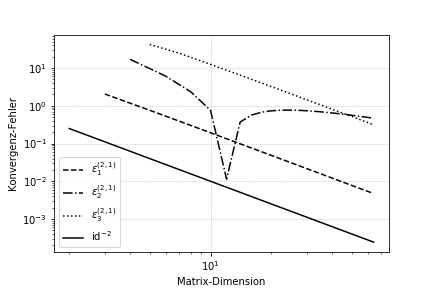
\includegraphics[width=65mm]{Aufgabe_2/images/plot_eigen_value_errors_general/plot_eigen_value_errors_general(n_max = 64, i_max = 3, c = (2, 1), parity = odd).png}
}
\subfloat[$c = (100, 1)$, $n \in 2 \N + 1$]{
  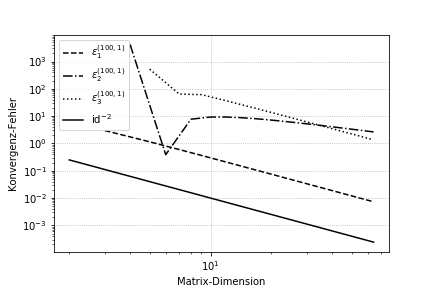
\includegraphics[width=65mm]{Aufgabe_2/images/plot_eigen_value_errors_general/plot_eigen_value_errors_general(n_max = 64, i_max = 3, c = (100, 1), parity = odd).png}
  \label{ungerade}
}
\hspace{0mm}
\caption{Konvergenz-Fehler der Eigenwerte von $B_n^{-1} A_n$, für $n = 2, \ldots, 64$ und}
\label{fig:Konvergenz-Fehler_EW_allgemein_besser}
\end{figure}

Wenn man für $c = (100, 1)$ gerade und ungerade betrachtet, so bemerkt man, dass $\epsilon_2^{(100, 1)}$ bei Abbildung \ref{gerade} konvergiert und $\epsilon_1^{(100, 1)}, \epsilon_3^{(100, 1)}$ bei Abbildung \ref{ungerade}. Dies lässt vermuten, dass im Allgemeinen die besten Approximationsstrategie ist, Teifolgen zu betrachten.

\begin{align*}
  \text{Benutze} \:
  \begin{cases}
    (\lambda_{i, n}^c)_{n \in 2 \N}     & \text{für} \: i \in 2 \N, \\
    (\lambda_{i, n}^c)_{n \in 2 \N + 1} & \text{für} \: i \in 2 \N + 1.
  \end{cases}
\end{align*}

Seien $\mathbf{v}^{(1, n), c}, \ldots, \mathbf{v}^{(n-1, n), c}$ die Eigenvektoren (modulo Konstante), zu den Eigenwerten $\lambda_{1, n}^c < \cdots < \lambda_{n-1, n}^c$, der Matrix $B_n^{-1} A_n$. Wir antizipieren ein weniger schönes Konvergenz-Verhalten, als das der Eigenvektoren der Matrizen $(A_n)_{n \in \N}$. Dennoch wurden die Eigenvektoren $\mathbf{v}^{(i, n_i), c}$, normiert bzgl. $\norm[\infty]{\cdot}$, geplottet, wobei

\begin{align*}
  c_{\mathrm{max}} & = 4, &
  c & \in \Bbraces{(c_0, c_1): c_0, c_1 = 1, \ldots, c_{\mathrm{max}}}, \\
  i & = 1, \ldots, 2 c_{\mathrm{max}}, &
  n_i & \in \Bbraces
  {
    2^{p_{\text{min}} + p_{\text{add}}}: \:
    p_{\text{min}} = \ceil{\log_2(i+1)}, \:
    p_{\text{add}} = 0, \ldots, 3
  } =: N_i.
\end{align*}

Dabei wurden die Vektoren $\Bbraces{\mathbf{v}^{(i, n), c}: n \in N_i}$ jeweils zu einem Bild zusammengefasst. Nachdem wir dadurch auf $128$ Bilder kommen, werden wir nicht alle herzeigen. Außerdem, sieht nur ein Bruchteil davon \enquote{schön} aus. \\

\begin{figure}[H]
  \centering
  \hspace{0mm}
  \subfloat[mit $i = 2$, $n = 4, 8, 16, 32$, und $c = (1, 4)$]{
    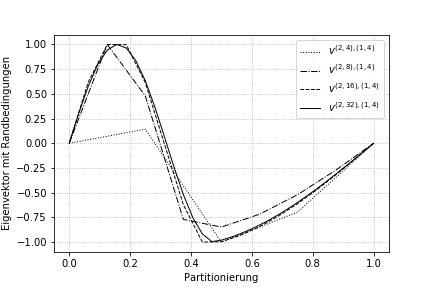
\includegraphics[width=65mm]{Aufgabe_2/images/plot_eigen_vectors_general/junk/plot_eigen_vectors_general(n_array = [4, 8, 16, 32], i = 2, c = (1, 4)).png}
  }
  \subfloat[mit $i = 6$, $n = 8, 16, 32, 64$, und $c = (1, 3)$]{
    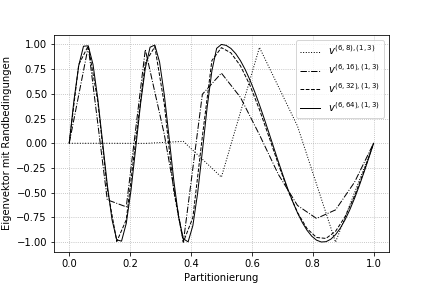
\includegraphics[width=65mm]{Aufgabe_2/images/plot_eigen_vectors_general/junk/plot_eigen_vectors_general(n_array = [8, 16, 32, 64], i = 6, c = (1, 3)).png}
  }
  \hspace{0mm}
  \subfloat[mit $i = 3$, $n = 4, 8, 16, 32$, und $c = (1, 2)$]{
    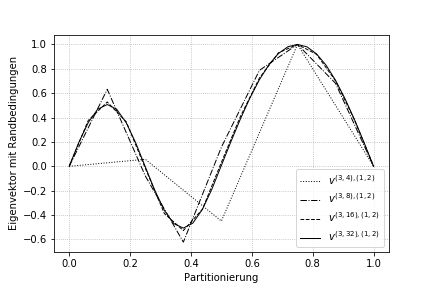
\includegraphics[width=65mm]{Aufgabe_2/images/plot_eigen_vectors_general/(1, 2), (2, 1)/plot_eigen_vectors_general(n_array = [4, 8, 16, 32], i = 3, c = (1, 2)).png}
  }
  \subfloat[mit $i = 5$, $n = 8, 16, 32, 64$, und $c = (2, 3)$]{
    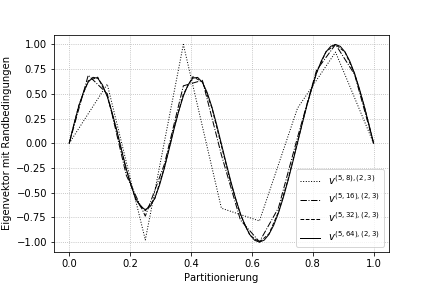
\includegraphics[width=65mm]{Aufgabe_2/images/plot_eigen_vectors_general/(2, 3), (3, 2)/plot_eigen_vectors_general(n_array = [8, 16, 32, 64], i = 5, c = (2, 3)).png}
  }
  \hspace{0mm}
  \caption{Eigenvektoren $\mathbf{v}^{(i, n), c}$ der Matrizen $B_n^{-1} A_n$}
  \label{fig:Eigenvektoren_general}
\end{figure}

Mit \enquote{schön} ist gemeint, dass die Grenzfunktionen bzgl. $n$ der Eigenvektoren $\mathbf{v}^{(i, n), c}$ seinen letzte (halbe) Schwingungs-Periode vollenden kann, bevor die nächste Ausbreitungsgeschwindigkeit übernimmt. Mit anderen Worten, die beiden Funktionshälften treffen sich an der $x$-Achse. Man fragt sich nun vielleicht, für welche Ausbreitungsgeschwindigkeiten $c$ und Eigenpaar-Nummerierung $i$ diese Grenzfunktionen \enquote{schön} aussehen. \\

Dazu bemerken wir zuerst, dass die selben Plots herauskommen, wenn $c^{(1)}, c^{(2)}$ bis auf eine Konstante übereinstimmen. Wegen der Normierung bzgl. $\norm[\infty]{\cdot}$, sieht man das durch hinschauen (auf $A \mathbf{v} = \lambda B \mathbf{v}$), also eigentilch auch bereits a priori.

\begin{align*}
  \mathbf{v}^{(i, n), c^{(1)}} = \mathbf{v}^{(i, n), c^{(2)}}, \:
  \text{für} \:
  c^{(1)} \equiv c^{(2)} \Mod \text{Konstante}.
\end{align*}

\begin{figure}[H]
  \centering
  \hspace{0mm}
  \subfloat[$c = (1, 2)$]{
    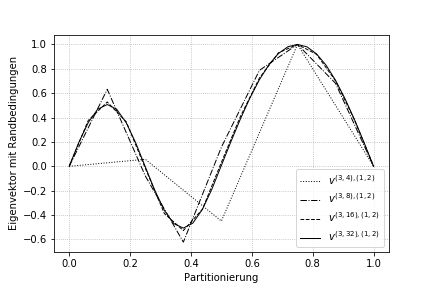
\includegraphics[width=65mm]{Aufgabe_2/images/plot_eigen_vectors_general/(1, 2), (2, 1)/plot_eigen_vectors_general(n_array = [4, 8, 16, 32], i = 3, c = (1, 2)).png}
  }
  \subfloat[$c = (2, 4)$]{
    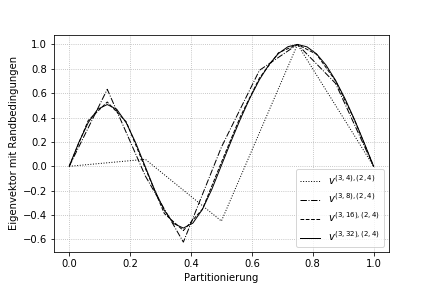
\includegraphics[width=65mm]{Aufgabe_2/images/plot_eigen_vectors_general/(1, 2), (2, 1)/plot_eigen_vectors_general(n_array = [4, 8, 16, 32], i = 3, c = (2, 4)).png}
  }
  \hspace{0mm}
  \caption{Eigenvektoren $\mathbf{v}^{(3, n), c}$ der Matrizen $B_n^{-1} A_n$, mit $n = 8, 16, 32, 64$ und}
  \label{fig:Eigenvektoren_general_Vielfache}
\end{figure}

A posteriori hingegen, bemerken wir, dass zwei Plots mit $(c_0, c_1)$ bzw. $(c_1, c_0)$ auch graphisch zusammenhängen. Die erste und zweite Hälft der Grenzfunktionen tauschen, wenn man zwischen den Plots wechselt. \\

\begin{figure}[H]
  \centering
  \hspace{0mm}
  \subfloat[$c = (1, 3)$]{
    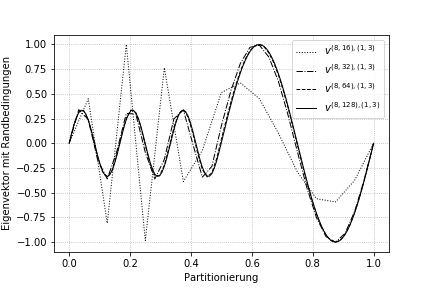
\includegraphics[width=65mm]{Aufgabe_2/images/plot_eigen_vectors_general/(1, 3), (3, 1)/plot_eigen_vectors_general(n_array = [16, 32, 64, 128], i = 8, c = (1, 3)).png}
  }
  \subfloat[$c = (3, 1)$]{
    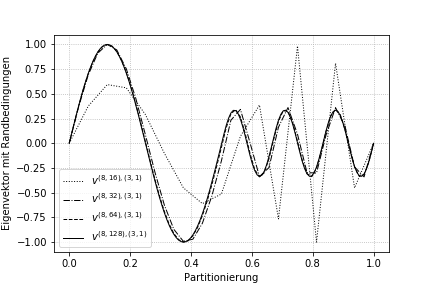
\includegraphics[width=65mm]{Aufgabe_2/images/plot_eigen_vectors_general/(1, 3), (3, 1)/plot_eigen_vectors_general(n_array = [16, 32, 64, 128], i = 8, c = (3, 1)).png}
  }
  \hspace{0mm}
  \caption{Eigenvektoren $\mathbf{v}^{(8, n), c}$ der Matrizen $B_n^{-1} A_n$, mit $n = 16, 32, 64, 128$ und}
  \label{fig:Eigenvektoren_general_vertauscht}
\end{figure}

Es sticht aber noch etwas Anderes ins Auge. Wenn man irgendeinen dieser Plots betrachtet, dann geht die Grenzfunktion genau dann durch den ausgezeichneten Punkt $(1/2, 0)$, wenn $\tilde{c_0} + \tilde{c_1} \: | \: i$, wobei $\tilde{c_0} : \tilde{c_1} = c_0 : c_1$ und $\tilde{c}$ vollständig gekürzt ist. \\

\begin{figure}[H]
  \centering
  \hspace{0mm}
  \subfloat[mit $i = 2$, $n = 4, 8, 16, 32$, und $c = (4, 4)$]{
    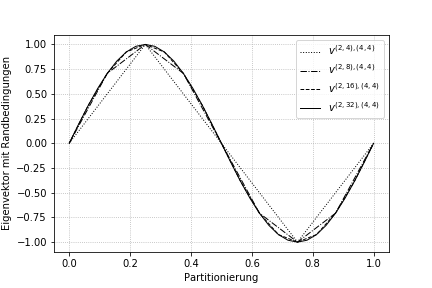
\includegraphics[width=65mm]{Aufgabe_2/images/plot_eigen_vectors_general/(1, 1)/plot_eigen_vectors_general(n_array = [4, 8, 16, 32], i = 2, c = (4, 4)).png}
  }
  \subfloat[mit $i = 4$, $n = 8, 16, 32, 64$, und $c = (1, 3)$]{
    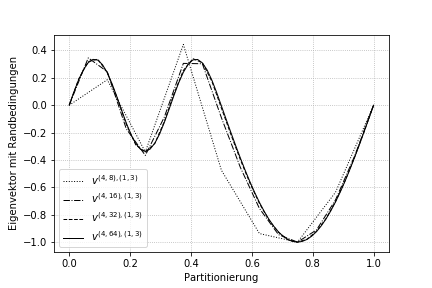
\includegraphics[width=65mm]{Aufgabe_2/images/plot_eigen_vectors_general/(1, 3), (3, 1)/plot_eigen_vectors_general(n_array = [8, 16, 32, 64], i = 4, c = (1, 3)).png}
    \label{subfig:double_trouble}
  }
  \hspace{0mm}
  \subfloat[mit $i = 8$, $n = 8, 16, 32, 64$, und $c = (1, 3)$]{
    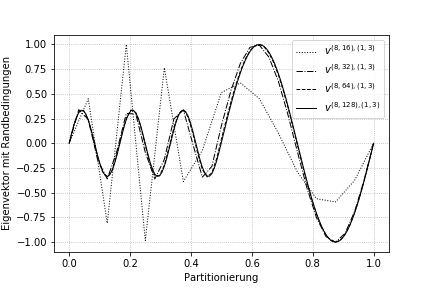
\includegraphics[width=65mm]{Aufgabe_2/images/plot_eigen_vectors_general/(1, 3), (3, 1)/plot_eigen_vectors_general(n_array = [16, 32, 64, 128], i = 8, c = (1, 3)).png}
  }
  \subfloat[mit $i = 7$, $n = 8, 16, 32, 64$, und $c = (3, 4)$]{
    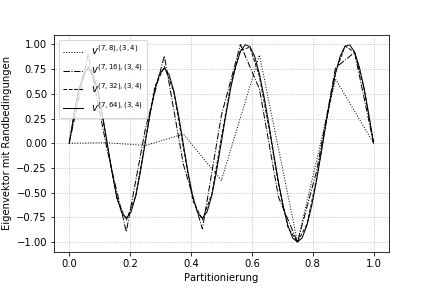
\includegraphics[width=65mm]{Aufgabe_2/images/plot_eigen_vectors_general/(3, 4), (4, 3)/plot_eigen_vectors_general(n_array = [8, 16, 32, 64], i = 7, c = (3, 4)).png}
  }
  \hspace{0mm}
  \caption{Eigenvektoren $\mathbf{v}^{(i, n), c}$ der Matrizen $B_n^{-1} A_n$}
  \label{fig:Eigenvektoren_general_nice}
\end{figure}

Das kann man heuristisch so begründen, dass die Ausbreitungsgeschwindigkeiten $c$, gemeinsam mit $i$, für die relativen Anzahlen der Schwingungsperioden verantwortlich sind; d.h, diese stehen diese im reziproken Verhältnis zu einander. Für $i = 4$, $c = (1, 3)$ aus Abbildung \ref{subfig:double_trouble} zum Beispiel, schwingt die erste Hälfte doppelt so schnell, wie die zweite. Dasselbe geschieht für $i = 8$, wobei die Grenzfunktion als Ganzes doppelt so schnell schwingt, wie bei $i = 4$. Durch dieses Zwischenspiel von $c$ und $i$, finden wir die meisten \enquote{schönen} Funktionen. \\

Was ist aber mit dem \enquote{künstlich verallgemeinerten} Fall $c = (1, 1) = \cdots = (c_{\mathrm{max}}, c_{\mathrm{max}})$, $i \in \N - 1$? Wieso sieht der so \enquote{schön} aus? Um eine Erklärung zu finden, verallgemeinern wir fröhlich weiter und betrachten die Material-Funktion $c = (c_0, \ldots, c_m) \in (\Q^+)^{m+1}$, wobei diese, analog zu \eqref{Material-Funktion}, bzgl. $1/(m+1)$ äquidistant zu verstehen ist.

\begin{align*}
  c(x) :=
  \begin{cases}
    c_0,   & x \in (0, 1/(m+1)) \\
    \vdots & \vdots \\
    c_m,   & x \in (m/(m+1), 1)
  \end{cases}
\end{align*}

Wir stellen fest, dass sich die naheliegende Verallgemeinerung der oberen Regel für diese Fälle gilt. Die Grenzfunktion geht genau dann durch die ausgezeichneten äquidistanten Punkte $\Bbraces{k/(m+1)}_{k=0}^{m+1}$, wenn $|\tilde{c}| := \tilde{c_0} + \cdots + \tilde{c_m} \: | \: i$, wobei $\tilde{c_0} : \cdots : \tilde{c_m} = c_0 : \cdots : c_m$ und $\tilde{c}$ als Ganzes vollständig gekürzt ist. \\

Tatsächlich gibt es im \enquote{künstlich verallgemeinerten} Fall mit beliebigem $i$ ein $m$, sodass für $c \in (\Q^+)^{m+1}$ gilt $|\tilde{c}| = m+1 \: | \: i$. Dieser Fall liefert übrigens, wegen der bereits angesprochenen Skalarmatrix, immer dasselbe Resultat.

\subsection{Vektor-Iteration}

Sei $\rho > 0$. Wir Verwenden die Vektor-Iteration angewendet auf das Eigenwertproblem

\begin{align} \label{geshiftetes_Eigenwertproblem}
  (A - \rho B)^{-1} B \tilde{\mathbf{v}} = \mu \tilde{\mathbf{v}}
\end{align}

mit den Matrizen $A$ und $B$ aus dem vorigen Unterkapitel. \\

Das macht man, weil die Vektor-Iteration in ihrer einfachsten Form, \verb|vector_iteration_simple|, nur den Eigenvektor mit dem betragsgrößten Eigenwert liefert. \\

\lstinputlisting
[language = Python]
{Aufgabe_2/python_code/vector_iteration_simple.py}
\vspace{10pt}

Es besteht ein Zusammenhang zwischen den Eigenpaaren $(\mu, \tilde{\mathbf{v}})$ und den Eigenpaaren $(\lambda, \mathbf{v})$ aus der vorigen Aufgabe. Für $\mu \neq 0$, ist dieser $\lambda = \rho + \frac{1}{\mu}$, weil dann

\begin{align*}
  A \mathbf{v} = \lambda B \mathbf{v}
  \Leftrightarrow
    A \mathbf{v} = \pbraces{\rho + \frac{1}{\mu}} B \mathbf{v}
  \Leftrightarrow
    B \mathbf{v} = \mu (A - \rho B) \mathbf{v}
  \Leftrightarrow
    (A - \rho B)^{-1} B \mathbf{v} = \mu \mathbf{v}.
\end{align*}

Bei der Vektor-Iteration wird der potentielle Eigenvektor $\mathbf{v}$ ständig normiert. Damit kann man wegen $A \mathbf{v} = \lambda \mathbf{v}$ sehr rasch auf den zugehörigen Eigenwert $\lambda$ kommen.

\begin{align*}
  \abraces{A \mathbf{v}, \mathbf{v}}
  = \abraces{\lambda \mathbf{v}, \mathbf{v}}
  = \lambda \norm{\mathbf{v}}^2
  = \lambda
\end{align*}

Jetzt können wir auch ein schlauereres Abbruch-Kriterium wählen. Die Vektor-Iteration soll terminieren, wenn die Änderung der Eigenwerte hinreichend klein ist. Die Implementierung, die diese Überlegungen beherzigt, folgt mit \verb|vector_iteration_unshifted|. \\

\lstinputlisting
[language = Python]
{Aufgabe_2/python_code/vector_iteration_unshifted.py}
\vspace{10pt}

Die untere Implementierung, \verb|vector_iteration_shifted|, der Vektor-Iteration des geshifteten Eigenwertproblems \eqref{geshiftetes_Eigenwertproblem}, ist ein gutes Beispiel eines sinnvollen Einsatzes der $LU$-Zerlegung. Diese ist zwar aufwändig, aber nachdem sie in jedem Iterationsschritt verwendet werden kann, zahlt sich dieser einmalige Aufwand aus. \\

\lstinputlisting
[language = Python]
{Aufgabe_2/python_code/vector_iteration_shifted.py}
\vspace{10pt}

Angenommen, wir wüssten bereits, dass all unsere Eigenwerte $\lambda_{1, n}^c < \cdots < \lambda_{n-1, n}^c \in \R^+$ reell und positiv sind. \verb|vector_iteration_simple| liefert uns den Eigenvektor mit dem betragsgrößten Eigenwert und \verb|vector_iteration_shifted| den Eigenvektor mit dem Eigenwert, der am nähesten bei $\rho$ liegt. Nun können wir mit einer binären Suche, ähnlich zum Bisektionsverfahren, alle Eigenwerte finden und ein eigenes \verb|np.linalg.eig| programmieren. \\

\lstinputlisting
[language = Python]
{Aufgabe_2/python_code/binary_search.py}
\vspace{10pt}

Das Abbruch-Kriterium ist aber anscheinend noch immer suboptimal, weil die damit berechneten Eigenwerte, sogar für \verb|tol = 1e-15|, nicht ganz denen von \verb|np.linalg.eig| entsprechen. \\

\begin{center}
\begin{tabular}{lrrrrr}
\toprule
{} &        2 &              3 &              4 &              5 &              6 \\
\midrule
1 &  20402.0 &      13.499662 &      21.329378 &      15.313793 &      20.048572 \\
2 &      NaN &  180004.500338 &   56813.374137 &      68.003831 &      96.940090 \\
3 &      NaN &            NaN &  344805.296478 &  180595.546136 &  102552.962297 \\
4 &      NaN &            NaN &            NaN &  750004.166956 &  392219.488916 \\
\bottomrule
\end{tabular}

\vspace{10pt}
\end{center}

Zum Vergleich, zeigen wir nochmal die Eigenwerte via \verb|np.linalg.eig|. Betrachtet man die Eigenwerte $\lambda_{3, 5}^{(100, 1)}, \lambda_{4, 6}^{(100, 1)}$, so merkt man, dass Ungenauigkeiten beim vorletzten Eigenpaar, d.h. Eigenpaar mit betragsmäßig zweitgrößten Eigenwert, auftreten, wenn $n$ groß ist. Offensichtlich, lässt sich diese Eigenwertsuche noch optimieren, das würde aber den Rahmen dieses Projektes sprengen. \\

\begin{center}
\begin{tabular}{lrrrrr}
\toprule
{} &        2 &              3 &              4 &              5 &              6 \\
\midrule
1 &  20402.0 &      13.499662 &      21.329378 &      15.313793 &      20.048572 \\
2 &      NaN &  180004.500338 &   56813.374144 &      68.017688 &      96.940091 \\
3 &      NaN &            NaN &  344805.296478 &  250012.501563 &  102552.962302 \\
4 &      NaN &            NaN &            NaN &  750004.166956 &  422576.319931 \\
\bottomrule
\end{tabular}

\vspace{10pt}
\end{center}

Zuletzt, wollen wir noch wissen, ob die Eigenwerte unserer Matrix $B_n^{-1} A_n$ tatsächlich alle positiv und reell sind. Sonst wäre der Algorithmus ja, aus mathematische Sicht, wertlos. Eine Möglichkeit bietet die explizite Darstellung von Eigenpaaren von Tridiagonalmatrizen. Wir wissen aber, dass das Gewünschte genau dann gilt, wenn $B_n^{-1} A_n$ positiv definit ist. Das können wir mit dem Hauptminoren-Kriterium locker überprüfen.

\begin{align*}
  A_n^\prime :=
  \begin{pmatrix}
     2 &  -1     &        &    \\
    -1 &  \ddots & \ddots &    \\
       &  \ddots & \ddots & -1 \\
       &         & -1     &  2
  \end{pmatrix}
\end{align*}

Zuerst berechnen wir die Determinante der Matrix $A_n^\prime$. Dazu induzieren wir $\det(A_n^\prime) = n$. Der Induktionsanfang, $n = 2, 3$, ist trivial. Für den Induktionsschritt muss man einmal nach der letzten Spalte und dann Zeile entwickeln (oder umgekehrt). \\

Nun gilt aber $A_n = \frac{1}{h^2} A_n^\prime$ und $\det(B_n^{-1}) > 0$, da $c_0, c_1 > 0$. Weil die Determinante dieser Matrizen bloß das Produkt ihrer Komponenten ist, sind alle Hauptminoren unserer Matrizen positiv. Sie sind also tatsächlich positiv definit. Deren Produkt und Vielfaches $A_n$ ist es also auch, weil

\begin{align*}
  0 < \mathbf{x}^\ast A \mathbf{x}, \mathbf{x}^\ast B \mathbf{x}
  \Rightarrow
  0 < \mathbf{x}^\ast A \mathbf{x} \mathbf{x}^\ast B \mathbf{x} =
  \mathbf{x}^\ast A \abraces{\mathbf{x}, \mathbf{x}} B \mathbf{x} =
  \mathbf{x}^\ast A \norm{\mathbf{x}}^2 B \mathbf{x}
  \Rightarrow
  0 < \mathbf{x}^\ast AB \mathbf{x}.
\end{align*}

\newpage
